\chapter{DUNE Detector Construction Management}
\label{vl:tc-dune_overview}


The purpose of this chapter is to provide an overview description of
the \dword{dune} \dword{fd} modules and their construction
management. The \dword{fd} consists of \SI{40}{\kilo\tonne} active
detector mass divided into four modules. Each module is contained in
its own cryostat and contains \nominalmodsize active mass and
$\sim$\SI{17}{\kilo\tonne} total mass. \dword{dune} has two detector designs:
\dword{sp} and \dword{dp}.  Full descriptions can be found in
\dword{sp} Volume~\volnumbersp\ and \dword{dp} Volume~\volnumberdp\
of this \dword{tdr}.

\section{DUNE Single Phase Far Detector Module}
\label{sec:fdsp-SP-module}

The \dword{sp} \dword{lartpc} is a \nominalmodsize module,
contributing to the full \SI{40}{\kilo\tonne} \dword{fd} fiducial
mass.  One \nominalmodsize \dword{spmod} is shown in
Figure~\ref{fig:DUNE_SP_model}.
\begin{dunefigure}[A \nominalmodsize SP module.]
{fig:DUNE_SP_model} 
{A \nominalmodsize DUNE FD SP module, showing alternating APAs,
    CPAs, FC and ground planes, detector support system, cryostat
    and cryogenics distribution.}
  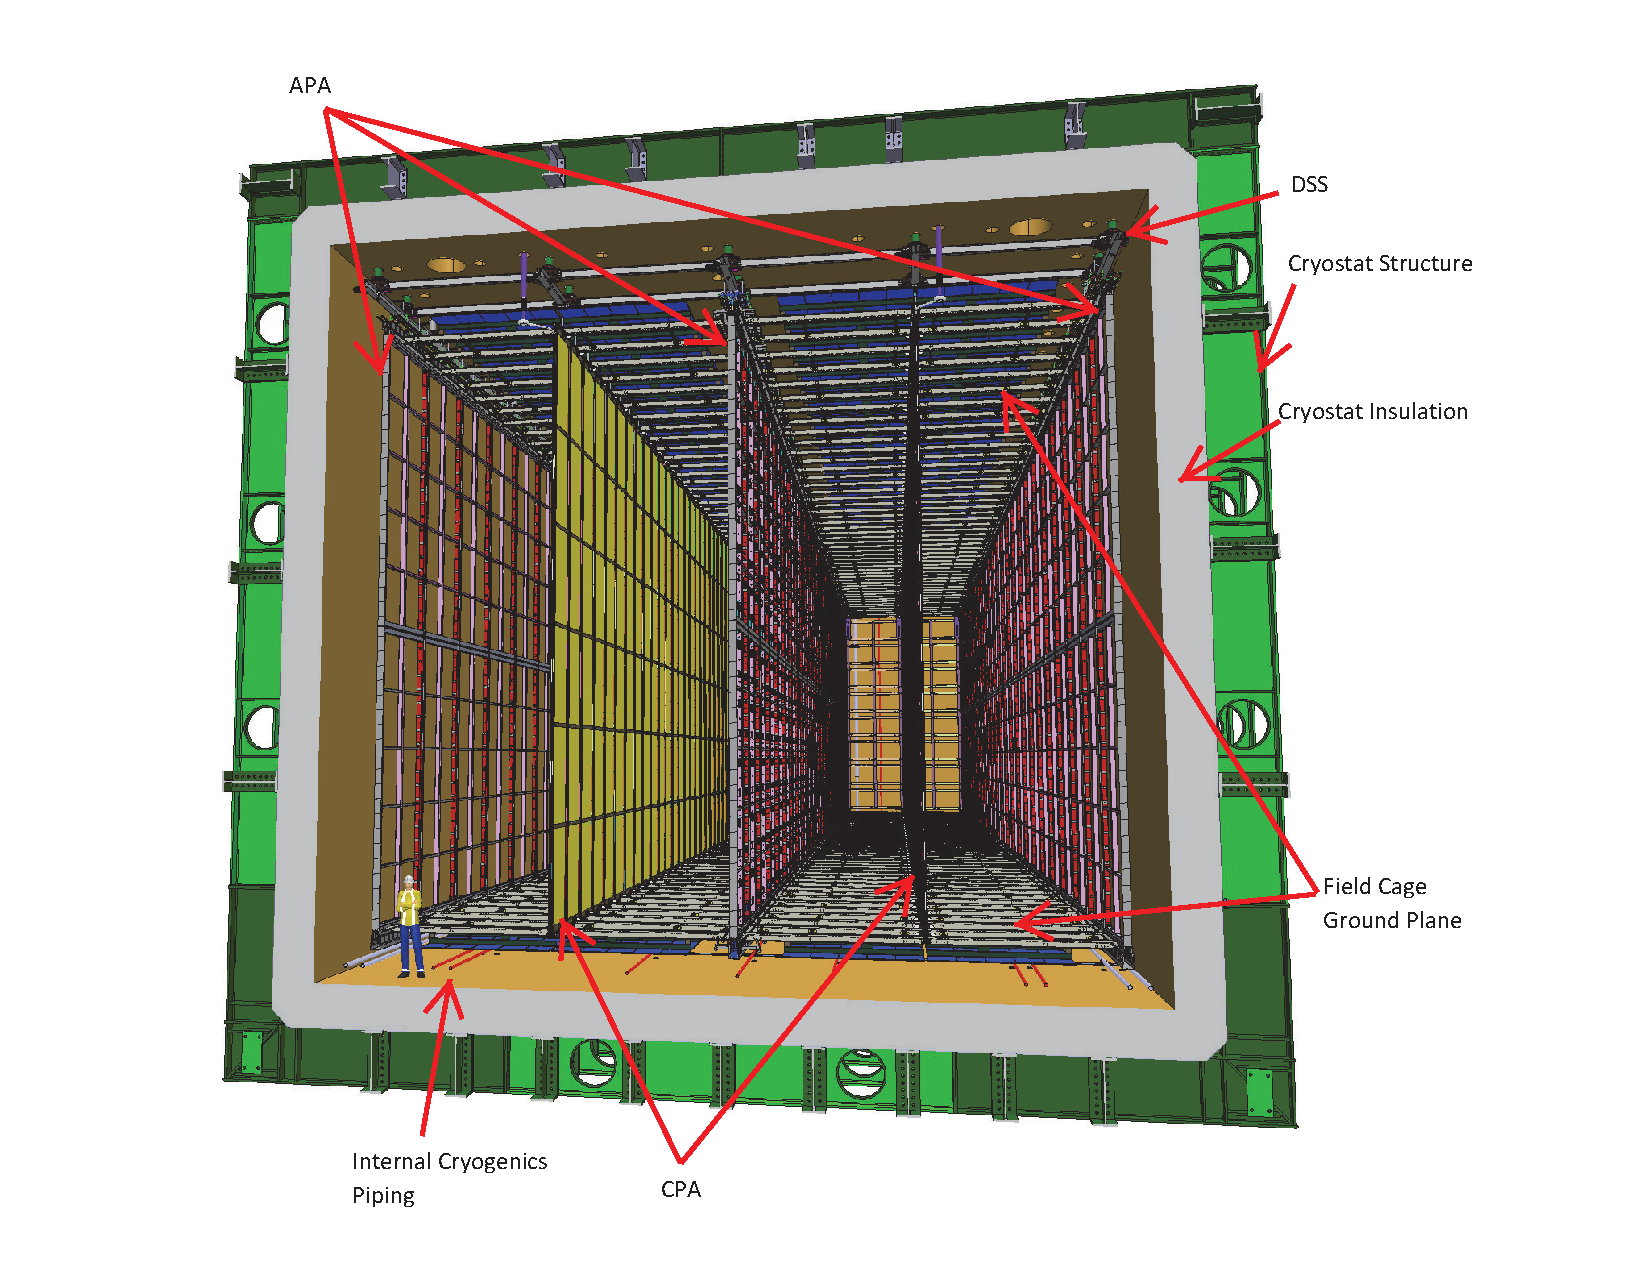
\includegraphics[width=0.99\textwidth]{DUNE_SP_model2}
\end{dunefigure} 

The module is contained in a cryostat as shown in
Figure~\ref{fig:dune-cryostat}.  Four drift volumes are created
between alternating \dword{apa} and \dword{cpa} walls on sides,
\dwords{fc} and \dwords{gp} on top and bottom, and two \dwords{ewfc}.
Each drift volume is \sptpclen long, \spmaxdrift wide and \tpcheight
high.  The entire assembly is supported from the roof of the cryostat
with \dword{dss}.

Each of the three \dword{apa} walls consists of an array of \num{25}
wide and \num{2} high individual \dwords{apa}, each with dimensions of
\SI{6.2}{\meter} high and \SI{2.32}{\meter} wide. There are \num{150}
\dwords{apa} in one module. Each \dword{apa} contains \num{10}
\dwords{pd}. Each of the two \dword{cpa} walls consists of an array of
\num{25} wide and \num{2} high \dword{cpa} panels. Two panels are
stacked to form planes, each with dimensions of \SI{12.1}{\meter} high
and \SI{1.16}{\meter} wide. There are \num{100} \dwords{cpa} in one
module.  \dword{cpa} walls are held at $-$\SI{180}{\kilo\volt}. With
\dword{apa} walls held close to ground, the result is a
\SI{511}{\volt/\centi\meter} gradient across the drift volume. The
drift in the \dword{spmod} is in the horizontal direction. The
\dword{lar} level is above the top set of \dwords{gp} and just below
the \dword{dss}.

Readout electronics are assembled on the \dwords{apa}. Cables from the
readout electronics and \dwords{pds} are routed to the cryostat roof
where they exit through a set of \num{75} feedthroughs. The cables are
connected to \dwords{wib} which are contained in \num{150}
\dwords{wiec} for \dwords{apa} and \num{75} crates for \dwords{pds}. Data
fibers from the \dwords{wiec} carry the data to \dword{daq} racks
inside the \dword{cuc}.

There are four \dword{hv} feedthroughs on top of the cryostat, two on
each end. In addition, there are feedthroughs for calibration,
instrumentation and cryogenics distribution. Power supplies, and
controls are located on top of the cryostat on a dedicated
mezzanine. Cryogenics equipment is also installed on a separate
mezzanine on top of the cryostat.

\section{DUNE Dual Phase Far Detector Module}
\label{sec:fdsp-DP-module}

Each \dword{dpmod} is a \nominalmodsize \dword{lartpc}, contributing
to the full \SI{40}{\kilo\tonne} \dword{fd} fiducial mass.  One
\nominalmodsize \dword{dpmod} is shown in
Figure~\ref{fig:DUNE_DP_model}.
\begin{dunefigure}[A \nominalmodsize DP module]{fig:DUNE_DP_model} {A \nominalmodsize DUNE   \dword{dpmod}.}
  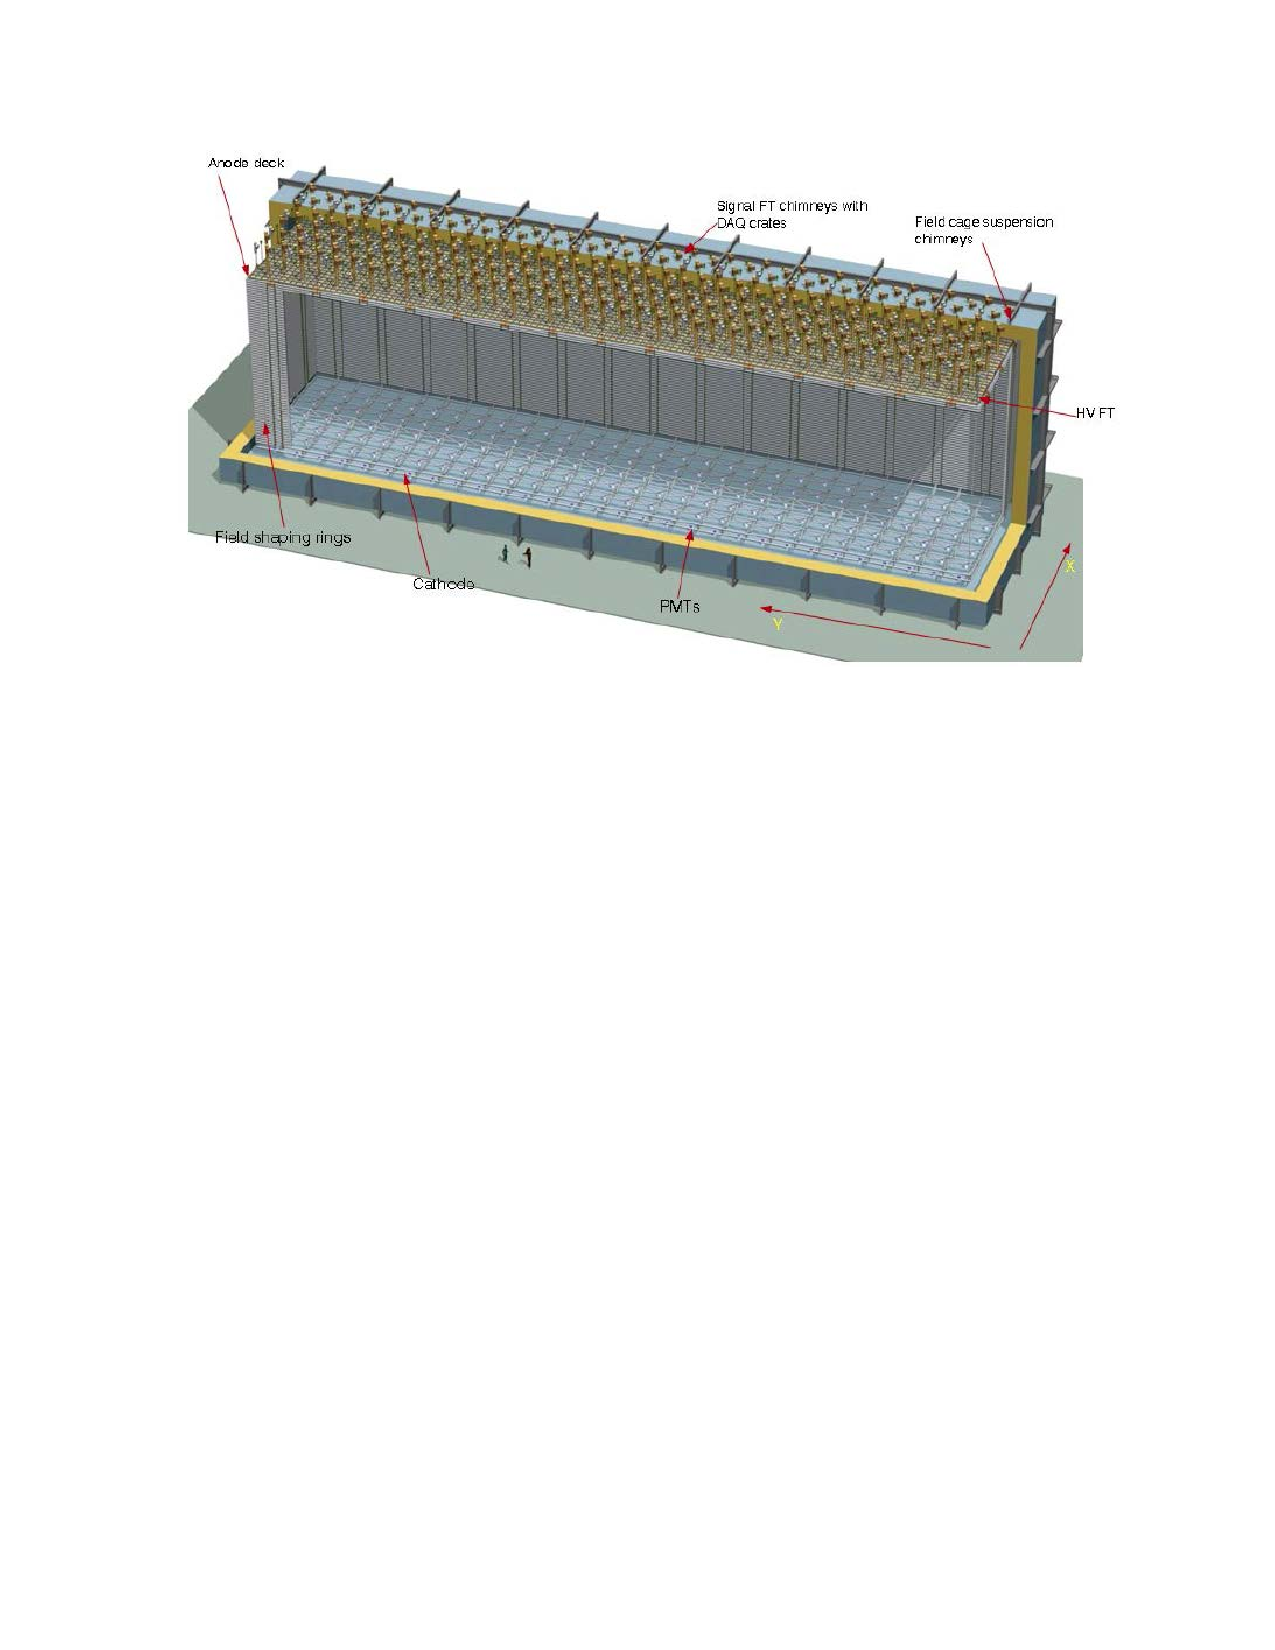
\includegraphics[width=0.8\textwidth]{DP-overview}
\end{dunefigure} 

Each \dword{dpmod} is contained in a cryostat with the same internal
dimensions as the \dword{spmod}, but with some variations in cryostat
penetrations.  The \dword{dpmod} consists of a single drift volume
with a vertical drift direction.

The drift volume is enclosed on the top by an array of \num{80}
\dwords{crp}, on the bottom by cathode planes and on the perimeter by
a \dwords{fc}. It is \dpmaxdrift in height with a \dpnominaldriftfield
gradient. The cathode is held at a potential of
\dptargetdriftvoltneg{}.  The \dword{dp} \dword{pds} consists of
\dpnumpmtch \dwords{pmt} at the bottom of the drift volume and is
integrated with the cathode planes.  The \dword{lar} level in
\dword{dpmod} is within the \dword{crp}, just above the collection
grid and below the anode readout plane. A gradient of
\SI{2}{\kilo\volt/\centi\meter} in this region is used to extract the
drift electrons from the liquid. A \dword{lem} with a gradient of
\SI{33}{\kilo\volt/\centi\meter} causes charge multiplication and
amplification of the charge that is then collected on the anode
consisting of two perpendicular %@D ????  set of two \dpstrippitch\si{mm}-pitch %3.125
readout strips.

The \dword{dp} \dword{dss} consists of a set of stainless steel
cables that are suspended from feedthroughs on top of the
cryostat. The cables are extended to the floor of the cryostat where
they are used to lift components to design height. In the case of
\dwords{crp}, there are three cables per panel with active height
control in order to position the panel precisely with respect to the
\dword{lar} surface.

The cryogenic \dword{fe} electronics is installed in the
\dwords{sftchimney} on the roof of the cryostat to process the
\dword{lartpc} signals. Each \dword{sftchimney} is coupled to a {utca}
crate to digitize the signals. These crates are connected via optical
fiber links to the \dword{daq} back end. Arrangement of equipment on
top of the cryostat is similar to the \dword{spmod}.

\section{DUNE Far Detector Consortia}
\label{sec:fdconsortia}

A total of eleven \dword{fd} consortia have been formed to cover 
the sub-systems required for the two detector types currently under
consideration.  In particular, three consortia (SP-APA, SP-TPC
Electronics and SP-Photon Detection) pursue subsystems specific to
the single-phase design and another three consortia (DP-CRP, DP-TPC
Electronics and DP-Photon Detection) pursue designs for \dword{dp}
specific subsystems.  An additional five consortia (HV System, \dword{daq},
Cryogenic Instrumentation/Slow Controls, Calibration, and Computing)
have responsibility for subsystems common to both detector
technologies.  Figure~\ref{fig:DUNE_consortia} shows the consortia 
associated with the \dword{fd} construction effort along with their 
current leadership teams.  
\begin{dunefigure}[DUNE consortia]{fig:DUNE_consortia}
  {\dword{dune} consortia organization. CL refers to consortium leader
    and TL refers to technical lead.}
  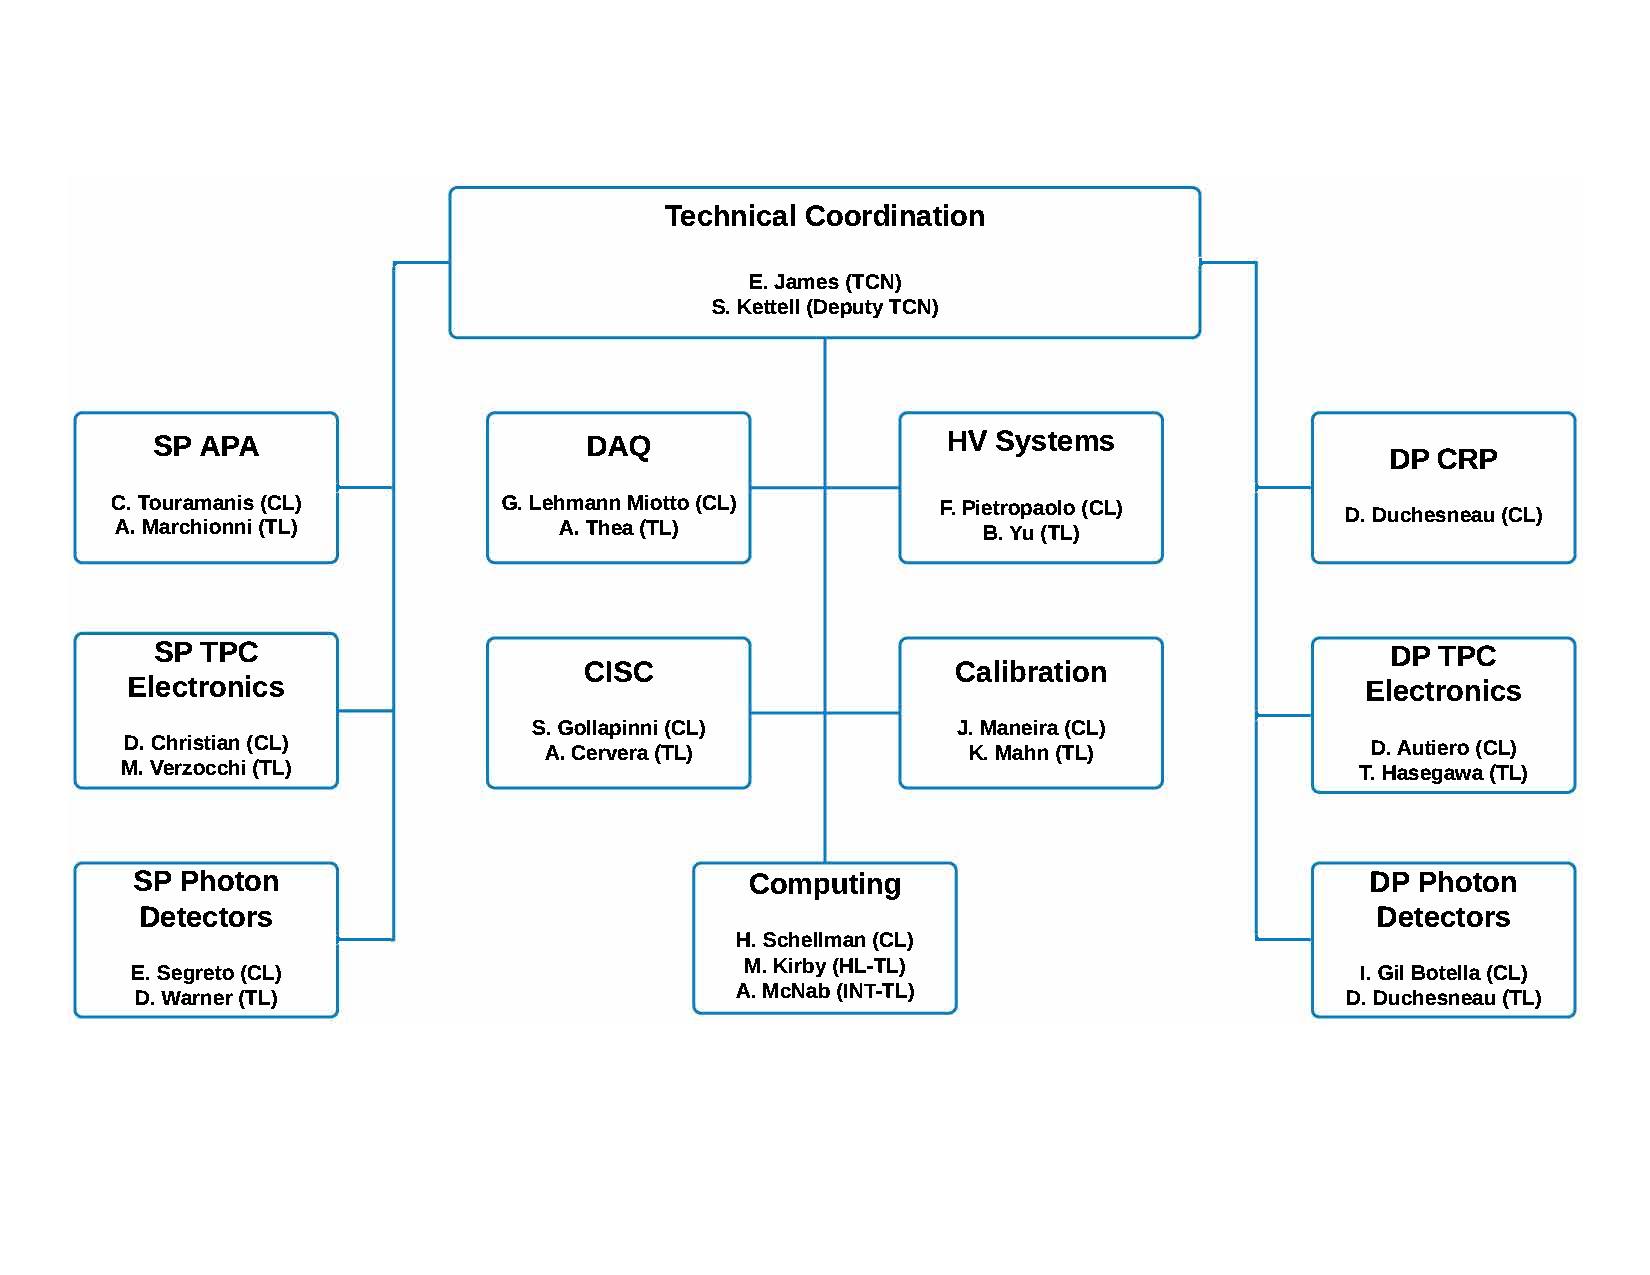
\includegraphics[width=0.99\textwidth]{Consortia_Org_Chart}
\end{dunefigure}

\section{Work Breakdown Structure (WBS)}
\label{sec:fdsp-coord-wbs}

The complete scope of the \dword{dune} construction project is captured in a 
\dword{wbs} to understand the distribution of deliverables between 
the consortia.  In combination with interface documentation, the 
\dword{wbs} is used to validate that all necessary scope is covered.  The 
\dword{wbs} is also used as a framework for building \dword{dune} 
detector cost estimates.

The highest-level layers of the \dword{dune} \dword{wbs} are summarized 
in Figure~\ref{fig:WBS_level2}.  At Level-1 the \dword{wbs} is broken down into 
six elements corresponding to the five \dword{dune} detector modules (four 
\dword{fd} and one \dword{nd}) and \dword{tc}.  The scope documented
here is fully contained within the \dword{tc}, first \dword{fd} module 
(\dword{sp}), and second \dword{fd} module (\dword{dp}) Level-1 elements.   
\begin{dunefigure}[DUNE WBS at level-2]{fig:WBS_level2}
  {High level \dword{dune} \dword{wbs} to level-2.}
  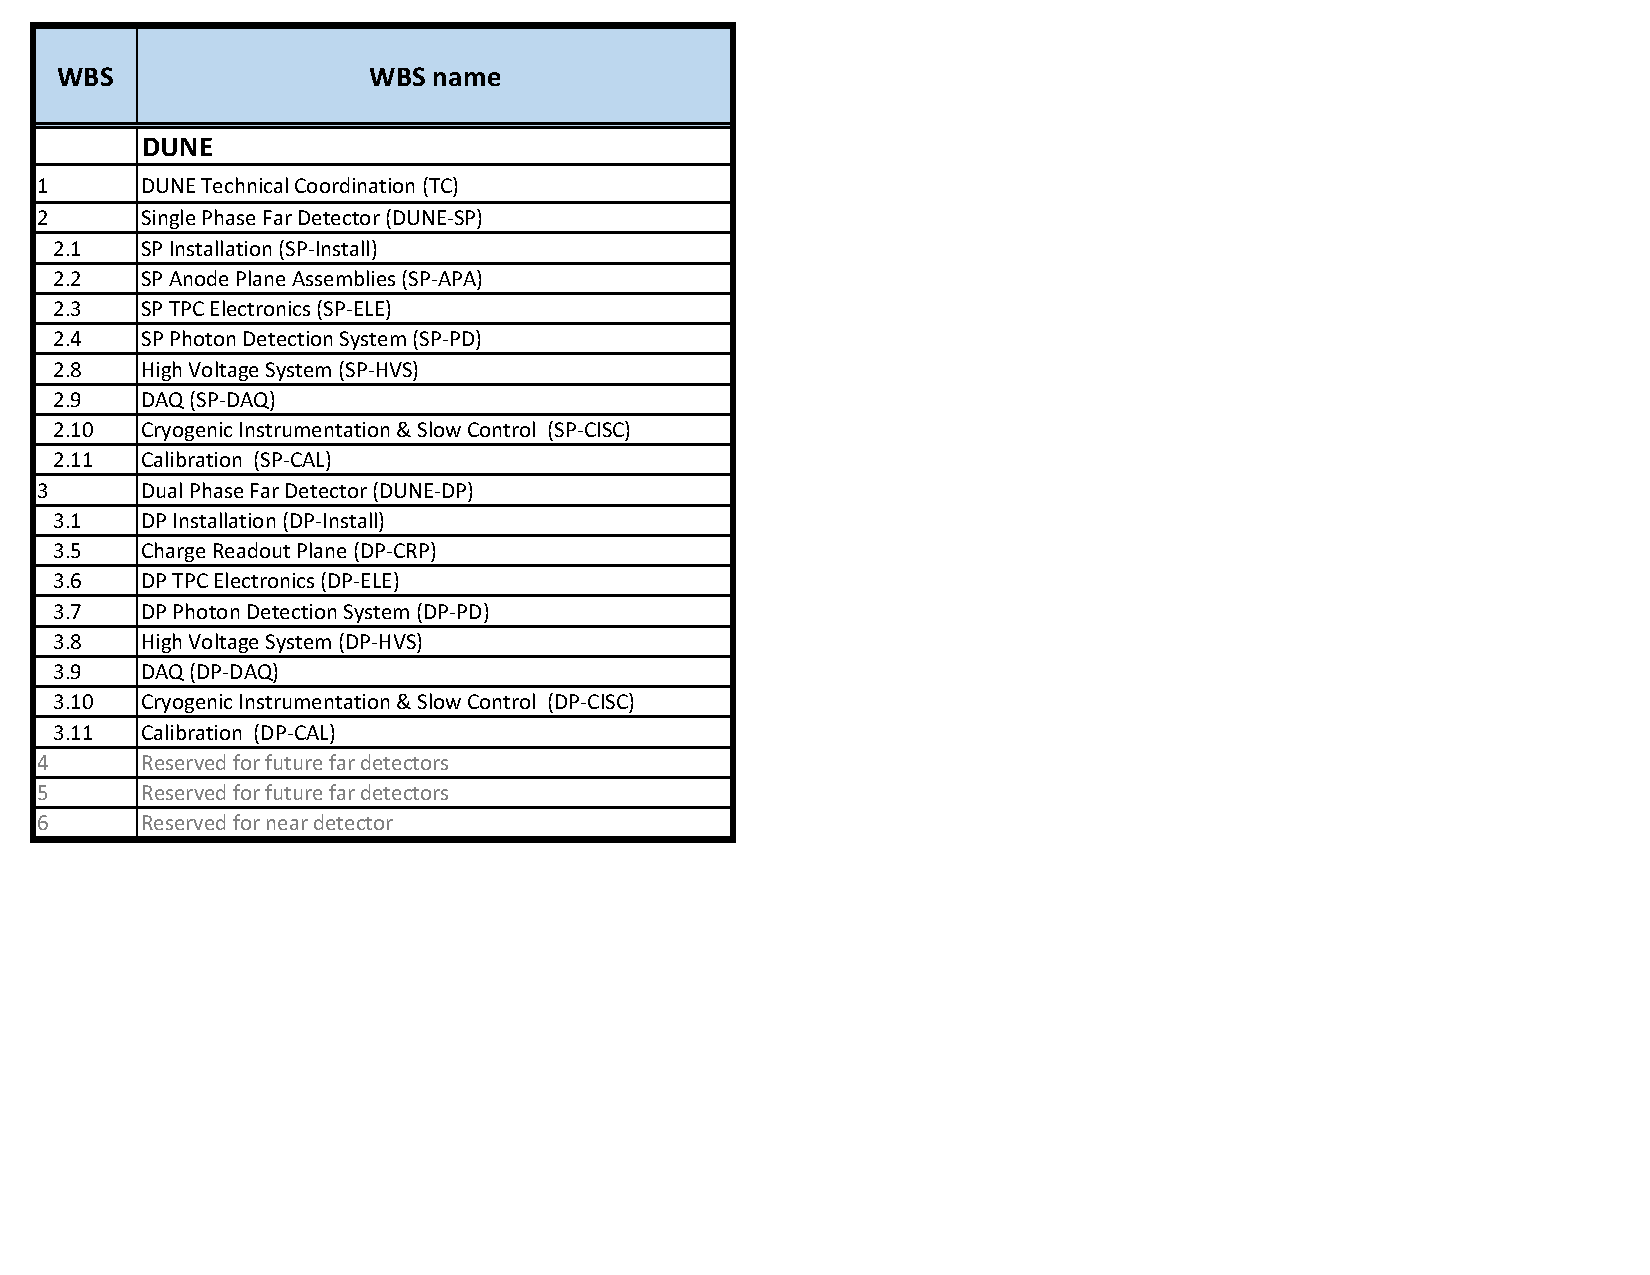
\includegraphics[width=0.75\textwidth]{WBS_level2_v2}
\end{dunefigure}

For the \dword{fd} module elements at Level-1, the \dword{wbs} breaks 
down at Level-2 into elements encompassing the deliverables provided by 
each consortium to that \dword{detmodule} along with an element containing 
common deliverables associated with the required detector installation 
and integration effort.  Since each consortium takes responsibility 
for a particular subsystem, this breakdown effectively corresponds to 
a division of deliverables across subsystems. 

The Level-3 breakdown of the Level-2 subsystem \dword{wbs} elements follow 
a common format that separates required activities into groupings defined 
roughly by their sequence in time.  A total of six elements are used as 
follows:     
\begin{enumerate}
  \item Management
  \item Physics and Simulation
  \item Design, Engineering and R\&D
  \item Production Setup
  \item Production
  \item Integration and Installation
\end{enumerate}
The groupings at Level-3 allow for the separation of costs associated
with \dword{core} and non-\dword{core} activities and also of the
costs associated with onetime and recurring activities in the case
where two identical detector modules are constructed.

Lower levels within these \dword{wbs} elements are determined by 
the responsible consortia and generally correspond at Level-4 to 
the different primary detector components from which each subsystem
is assembled.  This Level-4 structure is repeated under each of the 
Level-3 items to ensure that the full cost of each primary detector 
components can be rolled up over the sequence of activities defining 
their design, production, and installation.       

\section{DUNE Design Maturity}

The \dword{dune} project builds on significant development in previous
large \dword{lartpc} detectors (\dword{icarus} and \dword{microboone})
and on substantial development from \dword{lbne} and \dword{lbno}. One
of the most important elements that has significantly advanced the
project development is the successful construction of the
\dword{protodune} detectors and overwhelmingly successful operation of
\dword{pdsp}. These detectors use full-size \dword{dune} components
and processes. The construction of \dword{protodune} has established
teams, production lines, \dword{qa} and \dword{qc} processes,
installation, operation and performance of the final \dword{dune}
detectors.

Based on the success of \dword{protodune}, \dword{dune} has reached
advanced technical maturity, approaching (80\%). The designs have
significantly advanced from \dword{protodune} to \dword{dune}. Most
subsystems completed \dword{pdr} or 60\% reviews on design
modifications beyond \dword{protodune} in advance of the
\dword{tdr}. The overall level of design maturity is now
$\sim\,$90\%. The breakdown of the design maturity level for the
\dword{spmod} by subsystem is provided in
Table~\ref{tab:designmaturity}. The table shows the final \dword{dune}
design maturity at the time of \dword{protodune} and now at the time
of the \dword{tdr}, along with the estimated design effort or weight
of each subsystem.
\begin{dunetable}
  [SP module design maturity]
  {|p{0.1\linewidth}|rp{0.1\linewidth}|rp{0.25\linewidth}|rp{0.2\linewidth}|}
  {tab:designmaturity}
  {\dword{spmod} design maturity}
  System & Weight & \dword{protodune} & \dword{dune}   \\ \toprowrule
  DSS & 10\% & 75\% &  85\% \\ \colhline
  APA & 30\% & 85\% &  95\% \\ \colhline
  CE  & 20\% & 80\% &  90\% \\ \colhline
  PDS & 10\% & 50\% &  65\% \\ \colhline
  HVS & 15\% & 80\% &  95\% \\ \colhline
  DAQ & 10\% & 60\% &  80\% \\ \colhline
  CISC & 5\% & 80\% &  90\% \\ \colhline \colhline
  Total& 100\% & 76\% & 90\% \\ \colhline
\end{dunetable}

The \dword{apa} conceptual design was developed in 2010 and prototyped
at 40\% scale and again in the \dword{35t}. The version deployed in
\dword{pdsp} is close to that for the \dword{spmod} (85\%). The
\dword{ce} low-noise system design, including feedthroughs, cables and
grounding, was successfully prototyped at large scale in
\dword{microboone} and \dword{pdsp}, and is 90\% mature. The
\dword{fe} chip has gone through eight iterations and was successfully
demonstrated in \dword{microboone} and \dword{pdsp} (90\%). The
\dword{femb} has gone through a similar number of iterations and was
successfully demonstrated in \dword{pdsp} (80\%). The \dword{adc} chip
has evolved from a previous version used in \dword{cmos} 180~nm
technology that was tested to $-50^\circ$C. (70\%). Key elements of
the \dword{coldata} chip have been prototyped (70\%). The \dword{hv}
design has evolved from \dword{icarus}, \dword{microboone} and the
\dword{35t}.  It has been prototyped in subsequent runs of the
\dword{35t} and demonstrated in \dword{pdsp} (80\%). The \dword{pds}
\dword{xarapu} design has been prototyped at small scale and in
\dword{pdsp} (20\%). The mechanical design has been extensively
developed using the \dword{35t} detector and \dword{pdsp} (85\%). The
\dword{daq} \dword{artdaq} back end has been developed in several
experiments, including the \dword{35t} and \dword{pdsp}. The
\dword{daq} \dword{felix} \dword{fe} has been developed by
\dword{atlas} and prototyped in \dword{pdsp}.

The design maturity of the \dword{dp} detector technology is also
quite advanced. It builds on working noble liquid \dwords{tpc} for
dark matter and neutrinoless double beta decay experiments. A
significant benchmark is the operation of the \dword{wa105} at
\dword{cern}. The successful construction of \dword{pddp} and tests in
the cold box at \dword{cern} provide invaluable experience. A critical
test will be operation and analysis of \dword{pddp} at
\dword{cern}.

%%%%%%%%%%%%%%%%%%%%%%%%%%%%%%%%
